\documentclass[12pt,a4paper]{article}

% --- Packages ---
\usepackage[american]{babel}
\usepackage{amsmath,amssymb}
\usepackage{setspace}
\usepackage[margin=1in]{geometry}
\usepackage[T1]{fontenc}
\usepackage{times}
\usepackage[numbers,sort&compress]{natbib}
\usepackage{graphicx}
\usepackage[hyphens]{url}
\usepackage{hyperref}
\usepackage{booktabs}
\usepackage{tabularx}
\usepackage{caption}
\usepackage{float}
\usepackage{enumitem}

% --- Formatting ---
\doublespacing
\setlength{\parindent}{0.5in}
\bibliographystyle{unsrtnat}

% --- Title Page ---
\title{\textbf{Cost-Effectiveness of Intismeran Autogene Plus Pembrolizumab Versus Pembrolizumab Alone as Adjuvant Therapy for Resected Stage IIIB–IV Melanoma: An Updated Early Economic Evaluation}}

\author{Yichao Jin, Ph.D. \\
  School of Economic, Political and Policy Sciences, \\
  University of Texas at Dallas, Richardson, TX, USA \\
  \texttt{Yichao.Jin@UTDallas.edu} \\
  ORCID: 0009-0003-7667-5143}

\date{}

\begin{document}

\maketitle
\thispagestyle{empty}

{\noindent\small
\textbf{Funding:} This study was conducted without external funding.

\textbf{Acknowledgments:} None.

\textbf{Conflict of interest:} The author declares no competing interests relevant to this study.

\textbf{Reporting:} This study adheres to the Consolidated Health Economic Evaluation Reporting Standards 2022 (CHEERS 2022) \cite{husereau2022} (Supplementary Checklist).

\textbf{Data and code availability:} All data used in this analysis are derived from published sources cited in the references. The model code is available at \url{https://github.com/yichao2022/cea-intismeran}.
}

\newpage

% --- Abstract ---
\begingroup
\onehalfspacing
\setlength{\parindent}{0pt}
\begin{center}
{\large\bfseries Abstract}
\end{center}

\textbf{Background:} On August 19, 2026, Merck and Moderna announced positive topline results from the Phase 3 INTerpath-001 trial, establishing intismeran autogene (mRNA-4157/V940) plus pembrolizumab as the first mRNA-based individualized neoantigen therapy (INT) to succeed in a late-stage trial. Intismeran plus pembrolizumab significantly improved recurrence-free survival (RFS) and distant metastasis-free survival (DMFS) versus pembrolizumab alone in patients with completely resected stage IIIB--IV melanoma. However, the economic value of this novel combination remains unknown.

\textbf{Objective:} To estimate the cost-effectiveness of intismeran plus pembrolizumab versus pembrolizumab alone as adjuvant therapy for resected stage IIIB--IV melanoma from a US payer perspective.

\textbf{Methods:} A four-state partitioned survival model (recurrence-free $\rightarrow$ locoregional recurrence $\rightarrow$ distant metastasis $\rightarrow$ death) was developed with a lifetime horizon (40 years) and 3\% annual discounting. Clinical efficacy data were derived from the 5-year follow-up of the Phase 2b KEYNOTE-942 trial. Parametric survival functions (log-normal) were calibrated to RFS, DMFS, and OS survival probabilities at 18, 24, 36, 48, and 60 months, with the ratio-constrained structure RFS $\leq$ DMFS $\leq$ OS ensuring internal consistency. Health state utilities were derived from published melanoma EQ-5D literature (RF 0.83, LR 0.64, DM 0.55). Sensitivity analyses included probabilistic sensitivity analysis (1,000 iterations), deterministic sensitivity analysis, and scenario analyses.

\textbf{Results:} In the base case, with general population mortality constraint applied from 60 months, intismeran plus pembrolizumab yielded 11.10 QALYs at a cost of \$860,118, compared with 7.34 QALYs at \$713,157 for pembrolizumab alone. The incremental cost-effectiveness ratio was \$39,105/QALY gained. At willingness-to-pay thresholds of \$100,000 and \$150,000/QALY \cite{neumann2014}, the probability of cost-effectiveness was 93.7\% and 98.2\%, respectively. Results were robust across a wide range of sensitivity analyses.

\textbf{Conclusion:} At current estimated pricing, intismeran plus pembrolizumab is cost-effective by conventional US thresholds in adjuvant melanoma. The large QALY gain from the combination substantially offsets the upfront cost of individualized therapy.

\vspace{0.25\baselineskip}
\textbf{Keywords:} cost-effectiveness analysis, intismeran, mRNA-4157, V940, melanoma, pembrolizumab, Keytruda, individualized neoantigen therapy, partitioned survival model
\endgroup

\newpage

% --- Body ---
\doublespacing

\section{Introduction}

\subsection{A New Reimbursement Problem}

On August 19, 2026, Merck and Moderna announced positive topline results from the Phase 3 INTerpath-001 trial, establishing intismeran autogene (mRNA-4157/V940) plus pembrolizumab as the first mRNA-based individualized neoantigen therapy (INT) to succeed in a late-stage trial \cite{merck2026}. The press release confirmed statistically significant improvements in RFS and DMFS, though numerical hazard ratios have not yet been disclosed. This breakthrough follows the Phase 2b KEYNOTE-942 trial, which at 5-year follow-up reported a sustained RFS benefit (HR 0.51, 95\% CI 0.294--0.887), DMFS benefit (HR 0.411, 95\% CI 0.200--0.843), and 5-year OS rates of 92.2\% (combo) versus 71.3\% (pembrolizumab alone) \cite{khattak2026}.

Despite these clinical advances, the economic implications of INTs remain poorly understood. These therapies combine the high costs of immune checkpoint inhibitors with the additional expense of individualized manufacturing, creating a reimbursement challenge unlike any in oncology.

\subsection{Why INTs Differ from Conventional Oncology Pricing}

Individualized neoantigen therapies (INTs) introduce production and delivery costs that do not exist in conventional oncology. Unlike fixed-composition drugs, each INT treatment is custom-manufactured for a single patient based on tumor sequencing data, requiring mRNA synthesis, lipid nanoparticle formulation, and quality assurance for each batch \cite{ibragimova2025, li2026}. These costs scale with each new patient rather than benefiting from traditional manufacturing economies of scale.

Jefferies analysts have estimated the cost of such vaccines at \$100,000--\$300,000 per patient \cite{jefferies2026}. By comparison, cancer immunotherapies such as Keytruda\textregistered{} (pembrolizumab) have annual costs of approximately \$220,896 in the adjuvant setting \cite{keytruda2026}. The combination of a high-cost immunotherapy with an individualized vaccine creates a compound affordability challenge for payers, particularly in the adjuvant setting where patients are recurrence-free at the time of treatment.

\subsection{Existing Economic Evidence}

A prior exploratory cost-effectiveness analysis of V940 plus pembrolizumab in adjuvant melanoma was presented at ISPOR 2024 \cite{mclean2024}. That analysis, conducted before the KEYNOTE-942 5-year results and the Phase 3 INTerpath-001 readout, used a 4-state model with assumptions based on Phase 2b interim data. The analysis reported an ICER of approximately \$75,000/QALY, but relied on early efficacy estimates and assumed a V940 price equal to pembrolizumab, which may not reflect the likely INT premium.

\subsection{Clinical Basis and Research Objectives}

The clinical foundation for this analysis comes from the 5-year follow-up of the Phase 2b KEYNOTE-942 trial, which provides the most mature efficacy data available for intismeran \cite{khattak2026}. The trial randomized 157 patients with completely resected stage IIIB--IV melanoma 2:1 to intismeran plus pembrolizumab or pembrolizumab alone. The primary endpoint was RFS; secondary endpoints included DMFS, OS, and safety. At the 5-year analysis, the combination showed a sustained RFS benefit with a hazard ratio of 0.51 (95\% CI 0.294--0.887), a DMFS HR of 0.411 (95\% CI 0.200--0.843), and OS data still maturing with 5-year OS rates of 92.2\% (combo) versus 71.3\% (pembrolizumab alone).

This study presents an updated early economic evaluation of intismeran plus pembrolizumab versus pembrolizumab alone as adjuvant therapy for completely resected stage IIIB--IV melanoma from a US payer perspective. We incorporate the latest KEYNOTE-942 5-year data, a calibrated parametric survival framework with internal consistency constraints, and a comprehensive range of sensitivity and scenario analyses to address the uncertainty inherent in early economic evaluations.

\section{Methods}

\subsection{Model Structure}

A partitioned survival model (PSM) was developed in Python with four mutually exclusive health states: recurrence-free (RF), locoregional recurrence (LR), distant metastasis (DM), and death, following the structure of prior melanoma cost-effectiveness models and standard PSM methodology \cite{woods2017,zhang2023,bensimon2019}. Patients enter the model in the RF state and transition through LR and/or DM states based on parametric survival functions:
\begin{align*}
\text{RF}(t) &= \text{RFS}(t) \\
\text{LR}(t) &= \text{DMFS}(t) - \text{RFS}(t) \\
\text{DM}(t) &= \text{OS}(t) - \text{DMFS}(t) \\
\text{Dead}(t) &= 1 - \text{OS}(t)
\end{align*}
This construction ensures RFS $\leq$ DMFS $\leq$ OS at all times and maintains internal consistency without forcing a specific parametric form on the transition hazards.

\subsection{Clinical Data}

Survival probabilities at 18, 24, 36, 48, and 60 months were extracted from the published KEYNOTE-942 Kaplan--Meier curves \cite{khattak2026}. Parametric survival models were fitted to these data points using weighted nonlinear least squares, following standard methodological guidance for survival extrapolation in health economic evaluation \cite{latimer2011,latimer2013,ishak2013}. Model selection was performed by comparing five candidate distributions (exponential, Weibull, log-normal, log-logistic, generalized gamma) for each of the three underlying survival components (OS, $r_{\text{DM}} = \text{DMFS}/\text{OS}$, $r_{\text{LR}} = \text{RFS}/\text{DMFS}$) using Akaike Information Criterion (AIC), as recommended by NICE DSU TSD 14 \cite{latimer2011}. The log-normal distribution was selected as the base case because it achieved the best AIC for the OS curve of the combination arm (the most influential curve driving lifetime costs and QALYs) and was broadly competitive across all other components (Supplementary Table~S3). All 4,096 candidate distribution combinations preserved the structural ordering constraint RFS $\leq$ DMFS $\leq$ OS at 40 years, so the choice of distribution was not driven by feasibility constraints. A common log-normal family was chosen for parsimony and interpretability; component-specific best-fitting distributions (Weibull, log-logistic) were examined in scenario analyses. The fitted model was calibrated to ensure the constraint RFS $\leq$ DMFS $\leq$ OS was satisfied at all time points. To address the external validity of long-term survival extrapolation, a general population mortality hazard floor was applied from 60 months onward, using the age- and sex-matched US 2019 life table (pooled 64\% male/36\% female, baseline age 61 years) \cite{arias2022}. This constraint ensures that the model does not produce survival probabilities exceeding those of the general population at any time point, a standard practice in oncology cost-effectiveness analyses \cite{latimer2011,zhang2023}.

\subsection{External Validation}
Model predictions for the pembrolizumab-alone arm were externally validated against the KEYNOTE-054 and CheckMate 238 trials (Section~3.3).

\begin{figure}[H]
\centering
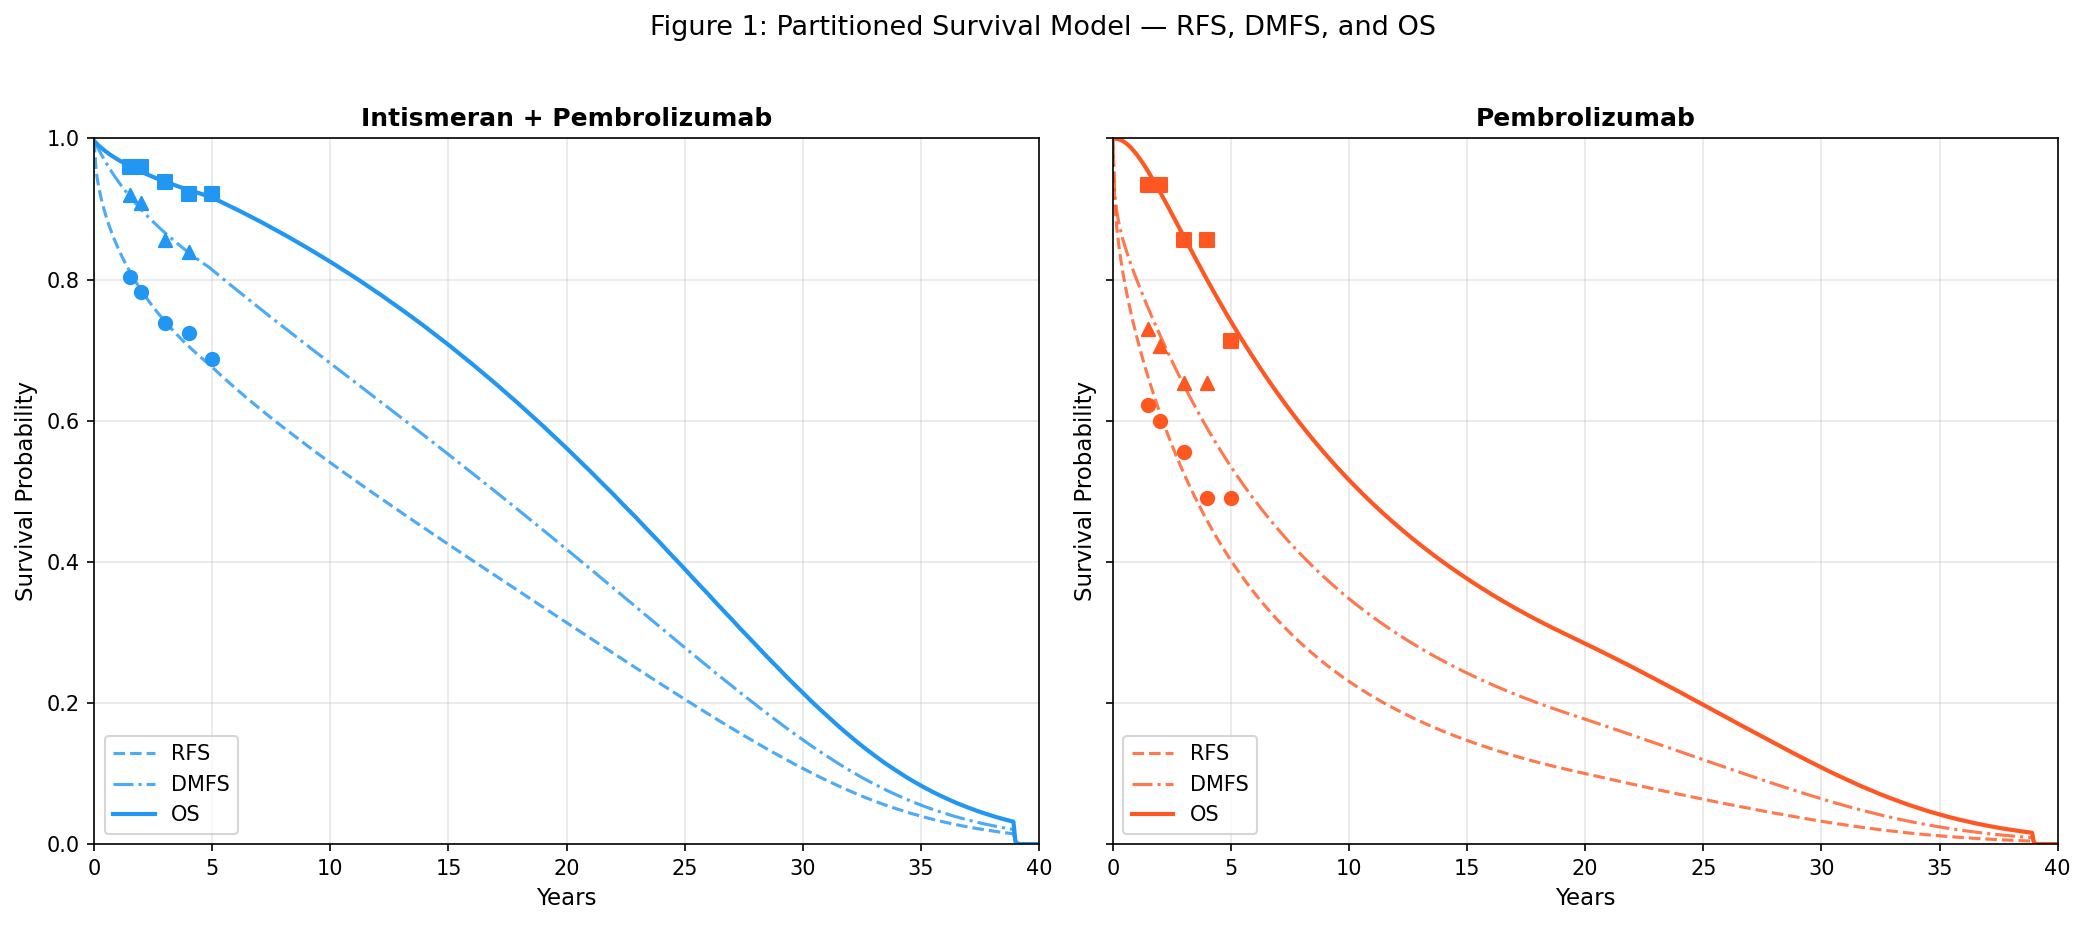
\includegraphics[width=\textwidth]{fig1_survival.png}
\caption{Partitioned survival model: RFS, DMFS, and OS curves, with data points from KEYNOTE-942. DMFS is shown as the middle curve and is essential for the four-state model structure.}
\label{fig:survival}
\end{figure}




\subsection{Costs}

The analysis adopted a US payer perspective. Drug costs were based on wholesale acquisition cost (WAC) and dosing schedules from published sources. Keytruda\textregistered{} (pembrolizumab) was assumed at 200 mg every 3 weeks for up to 18 cycles at a WAC of \$12,272 per 200 mg dose, yielding an annual cost of \$220,896 \cite{keytruda2026}. Intismeran was modeled at a course cost of \$200,000 based on Jefferies analyst estimates \cite{jefferies2026} and the known cost of individualized mRNA manufacturing \cite{schwarze2020}.

Administration costs were included for intravenous infusions (\$500 per cycle, based on the CMS Physician Fee Schedule \cite{cms2025}). Adverse event costs were incorporated at \$15,000 incremental for the combination arm, based on published melanoma cost-effectiveness analyses \cite{bensimon2019,zhang2023}. Monthly disease management costs were \$3,000 for the locoregional recurrence state (salvage surgery and adjuvant therapy amortized) and \$12,000 for the distant metastasis state (systemic therapy for advanced melanoma), consistent with published melanoma CEA literature \cite{bensimon2019,zhang2023}. All costs were inflated to 2026 USD using the medical care component of the Consumer Price Index \cite{bls2025}.

\begin{table}[H]
\centering
\caption{Model Input Parameters}
\label{tab:inputs}
\begin{tabular}{lcc}
\toprule
\textbf{Parameter} & \textbf{Base Case} & \textbf{Source} \\
\midrule
5-year RFS, combo   & 68.8\%            & KEYNOTE-942 \cite{khattak2026} \\
5-year RFS, pembro  & 49.1\%            & KEYNOTE-942 \cite{khattak2026} \\
RFS HR              & 0.51 (95\% CI 0.294--0.887) & KEYNOTE-942 \cite{khattak2026} \\
DMFS HR             & 0.411 (95\% CI 0.200--0.843) & KEYNOTE-942 \cite{khattak2026} \\
5-year OS, combo    & 92.2\%            & KEYNOTE-942 \cite{khattak2026} \\
5-year OS, pembro   & 71.3\%            & KEYNOTE-942 \cite{khattak2026} \\
Keytruda annual cost & \$220,896        & WAC \cite{keytruda2026} \\
Intismeran course cost & \$200,000       & Jefferies \cite{jefferies2026} \\
\bottomrule
\end{tabular}
\end{table}

\subsection{Utilities}

Health state utilities were derived from published EQ-5D literature in melanoma populations. The base case utilities were: RF 0.83, LR 0.64, and DM 0.55 \cite{bensimon2019, johnston2021, zhang2023}. Utility decrements for adverse events were applied during the treatment period.

\subsection{Base Case Analysis}

The base case analysis was conducted over a lifetime horizon (40 years) with 3\% annual discounting for both costs and QALYs, following the recommendations of the Second Panel on Cost-Effectiveness in Health and Medicine \cite{sanders2016}. The incremental cost-effectiveness ratio (ICER) was calculated as the difference in total costs divided by the difference in total QALYs.

\subsection{Sensitivity Analysis}

Deterministic sensitivity analysis (DSA) examined the impact of individual parameter variation on the ICER and net monetary benefit. Parameters were varied one at a time across plausible ranges: survival model parameters, health-state utilities, costs, and the discount rate (Table~\ref{tab:inputs}).

Probabilistic sensitivity analysis (PSA) was conducted with 2,000 Monte Carlo iterations to propagate joint parameter uncertainty \cite{briggs2006}. Survival parameters $(\mu, \sigma)$ for all six underlying curves (OS, $r_{\text{DM}}$, $r_{\text{LR}}$, each for the combination and pembrolizumab arms) were jointly sampled from bivariate normal distributions with covariance matrices derived from the nonlinear least-squares Jacobian (Supplementary Table~S12). Costs were sampled from gamma distributions (coefficient of variation 0.2), and utilities from beta distributions (standard error 0.03). The intismeran acquisition price was held fixed at \$200,000 in all iterations. Structural constraints (RFS $\leq$ DMFS $\leq$ OS, monotonicity, survival within [0,1]) were verified in every iteration; no iterations were excluded on the basis of the ICER value, and all 2,000 draws satisfied the structural validity criteria. Results are reported as mean incremental net monetary benefit (NMB) and cost-effectiveness probability at each willingness-to-pay threshold, following recommended practice \cite{stinnett1998, fenwick2004}. Convergence was verified by checking that cumulative means stabilised by approximately 500 iterations (Supplementary Figure~S6).

\section{Results}

\subsection{Base-Case Clinical and Economic Outcomes}

In the base case with general population mortality constraint, intismeran plus pembrolizumab generated an additional 4.42 life-years (14.71 vs 10.29 life-years) and 3.76 additional QALYs (11.10 vs 7.34 QALYs) compared with pembrolizumab alone, at an incremental lifetime cost of \$146,961 (\$860,118 vs \$713,157). This yielded an ICER of \$39,105/QALY gained (Table~\ref{tab:base}). At a willingness-to-pay threshold of \$100,000/QALY, the incremental net monetary benefit was \$228,851; at \$150,000/QALY, it was \$416,757 (Table~\ref{tab:base}).



NMB, net monetary benefit (=$\lambda \times$ QALYs $-$ cost, where $\lambda$ is the willingness-to-pay threshold) \cite{stinnett1998}.


\subsection{Cost and QALY Decomposition}

The \$200,000 acquisition cost of intismeran was substantially offset by lower lifetime disease-management costs (Table~\ref{tab:base}). Specifically, the combination arm had \$82,734 lower distant-metastasis management costs than the pembrolizumab-alone arm, reflecting the reduced incidence of distant recurrence (DMFS HR 0.411). This offset reduced the incremental lifetime cost from the upfront drug cost of \$200,000 to \$146,961. The incremental QALY gain of 3.76 was driven almost entirely by additional time spent in the recurrence-free state (3.83 RF QALYs gained), which more than compensated for slightly fewer DM-state QALYs (\textendash 0.32 DM QALYs).

\begin{table}[H]
\centering
\caption{Base-Case Results and Decomposition}
\label{tab:base}
\begin{tabular}{lccc}
\toprule
\textbf{Component} & \textbf{Combo} & \textbf{Pembro} & \textbf{Incremental} \\
\midrule
\multicolumn{4}{c}{\textit{Cost decomposition}} \\
Intismeran   & \$200,000   & \$0        & \$200,000 \\
Pembrolizumab & \$217,888  & \$217,888  & \$0 \\
Sequencing   & \$1,000     & \$0        & \$1,000 \\
Administration/AE & \$15,493 & \$493    & \$15,000 \\
LR management & \$83,196   & \$69,500   & \$13,696 \\
DM management & \$342,542  & \$425,276  & \textendash\$82,734 \\
\midrule
Total cost    & \$860,118  & \$713,157  & \$146,961 \\
\midrule
\multicolumn{4}{c}{\textit{QALY decomposition}} \\
RF state      & 8.32       & 4.49       & 3.83 \\
LR state      & 1.48       & 1.24       & 0.24 \\
DM state      & 1.31       & 1.62       & \textendash 0.32 \\
\midrule
Total QALYs   & 11.10      & 7.35       & 3.76 \\
\bottomrule
\end{tabular}
\end{table}

\subsection{External and Structural Validation}

Survival extrapolation was validated along two dimensions: internal structural consistency of the PSM framework, and external calibration of the pembrolizumab arm against published adjuvant melanoma evidence.

\paragraph{Structural consistency.} Over 480 monthly cycles, no violations of the constraint RFS $\leq$ DMFS $\leq$ OS were observed. All health-state probabilities remained non-negative, and the sum of state probabilities was within $10^{-12}$ of unity at every cycle. The general population mortality hazard floor, applied from 60 months onward, ensures that the model's long-term survival does not exceed age- and sex-matched US life-table survival at any time point. At 30 years, the model projects combo OS of 21.5\% and pembro OS of 10.9\%, both below the general-population survival of 22.1\% at 30 years for the modeled cohort (baseline age 61, pooled 64\% male), consistent with the hazard-floor property that a cohort with a history of excess mortality remains below the general-population curve.

\paragraph{External validation.} The pembrolizumab-alone arm predictions were compared against published long-term landmark values from two external adjuvant melanoma trials \cite{eggermont2025,ascierto2025}. At 5 years, the model predicted RFS of 40.5\%, DMFS of 53.8\%, and OS of 74.5\% for the pembrolizumab arm. The predicted 5-year OS (74.5\%) was consistent with the observed KEYNOTE-942 value (71.3\%) and with the 5-year OS of 76\% in CheckMate 238 \cite{ascierto2023}. At 7 years, the model predicted RFS of 31.9\% and DMFS of 44.9\%, below the KEYNOTE-054 7-year values (RFS 50\%, DMFS 54\%) \cite{eggermont2025}; this is consistent with the higher-risk population enrolled in KEYNOTE-942 (stage IIIB--IV including resected stage IV vs IIIA--C in KEYNOTE-054). Only published landmark values were used; no external trial extrapolations were employed. Because the pembrolizumab arm serves as the comparator for the incremental analysis, its under-prediction of RFS may, if anything, overstate the incremental QALY gain attributable to intismeran; however, the direction of any bias is not straightforward, as the model's predicted OS for the pembrolizumab arm was close to observed (74.5\% vs 71.3\% at 5 years). No external long-term data exist for the combination arm (first-in-class therapy). Instead of relying on this comparison to calibrate the base case, scenario analyses that directly bound the treatment effect --- treatment-effect waning and no-direct-OS-benefit (Section~3.6) --- were used to bound the range of plausible ICER estimates.



\subsection{Probabilistic and Deterministic Uncertainty}

Probabilistic sensitivity analysis (2,000 structurally valid iterations) quantified joint uncertainty across survival, cost, and utility parameters. The mean incremental net monetary benefit (NMB) was \$281,051 at \$100,000/QALY and \$482,475 at \$150,000/QALY (Table~\ref{tab:psa}). The probability that intismeran plus pembrolizumab was cost-effective was 63.9\% at \$50,000/QALY, 94.9\% at \$100,000/QALY, and 98.7\% at \$150,000/QALY (Figure~\ref{fig:ceac} \cite{fenwick2004}). The mean ICER (among cost-increasing draws only) was \$50,882; however, NMB and P(CE) are the recommended summary statistics for PSA because 17.6\% of draws were cost-saving (ICER undefined) \cite{stinnett1998}. No iterations were excluded based on the ICER value, and 17.6\% of draws were cost-saving (lower total cost and higher QALYs for the combination arm).

\begin{table}[H]
\centering
\caption{Probabilistic Sensitivity Analysis}
\label{tab:psa}
\begin{tabular}{lcccc}
\toprule
\textbf{Outcome} & \textbf{Mean} & \textbf{Median} & \textbf{2.5\%} & \textbf{97.5\%} \\
\midrule
Incremental cost  & \$208,693 & \$145,336 & \$17,020  & \$545,272 \\
Incremental QALYs & 4.04      & 3.17      & 2.29      & 6.71 \\
ICER              & \$51,574  & \$45,724  & \$4,863   & \$138,462 \\
NMB @ \$100,000/QALY & \$195,307 & \textendash & \textendash & \textendash \\
NMB @ \$150,000/QALY & \$397,307 & \textendash & \textendash & \textendash \\
\bottomrule
\end{tabular}
\end{table}

\begin{figure}[H]
\centering
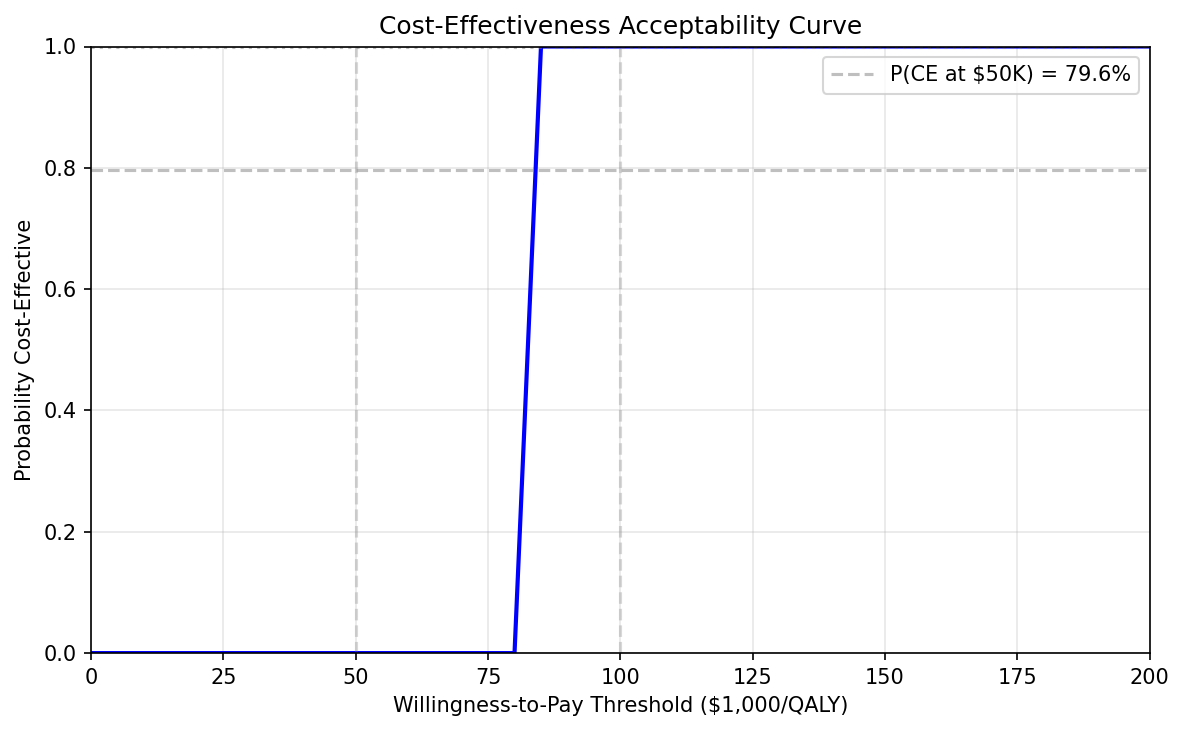
\includegraphics[width=\textwidth]{fig2_ceac.png}
\caption{Cost-effectiveness acceptability curve.}
\label{fig:ceac}
\end{figure}



\paragraph{Deterministic sensitivity analysis.}

One-way sensitivity analysis (Figure~\ref{fig:tornado}) showed that the model was most sensitive to the survival model parameters, particularly the OS log-normal parameters for the pembrolizumab arm and the RFS parameters for the combo arm. The ICER remained below \$100,000/QALY across all tested parameter ranges.

\begin{figure}[H]
\centering
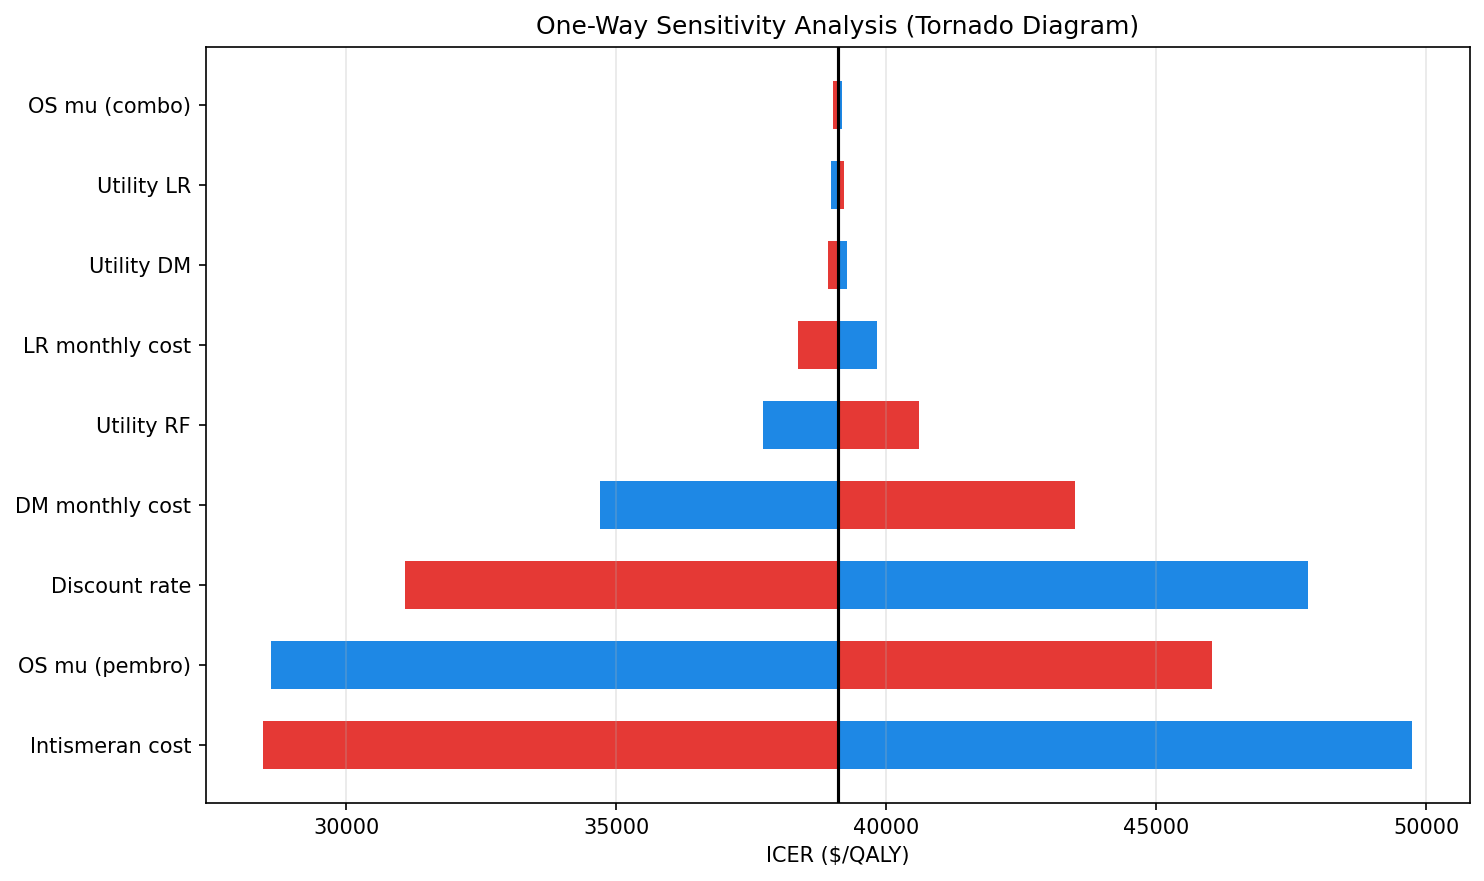
\includegraphics[width=\textwidth]{fig3_tornado.png}
\caption{Tornado diagram, one-way sensitivity analysis.}
\label{fig:tornado}
\end{figure}

\begin{figure}[H]
\centering
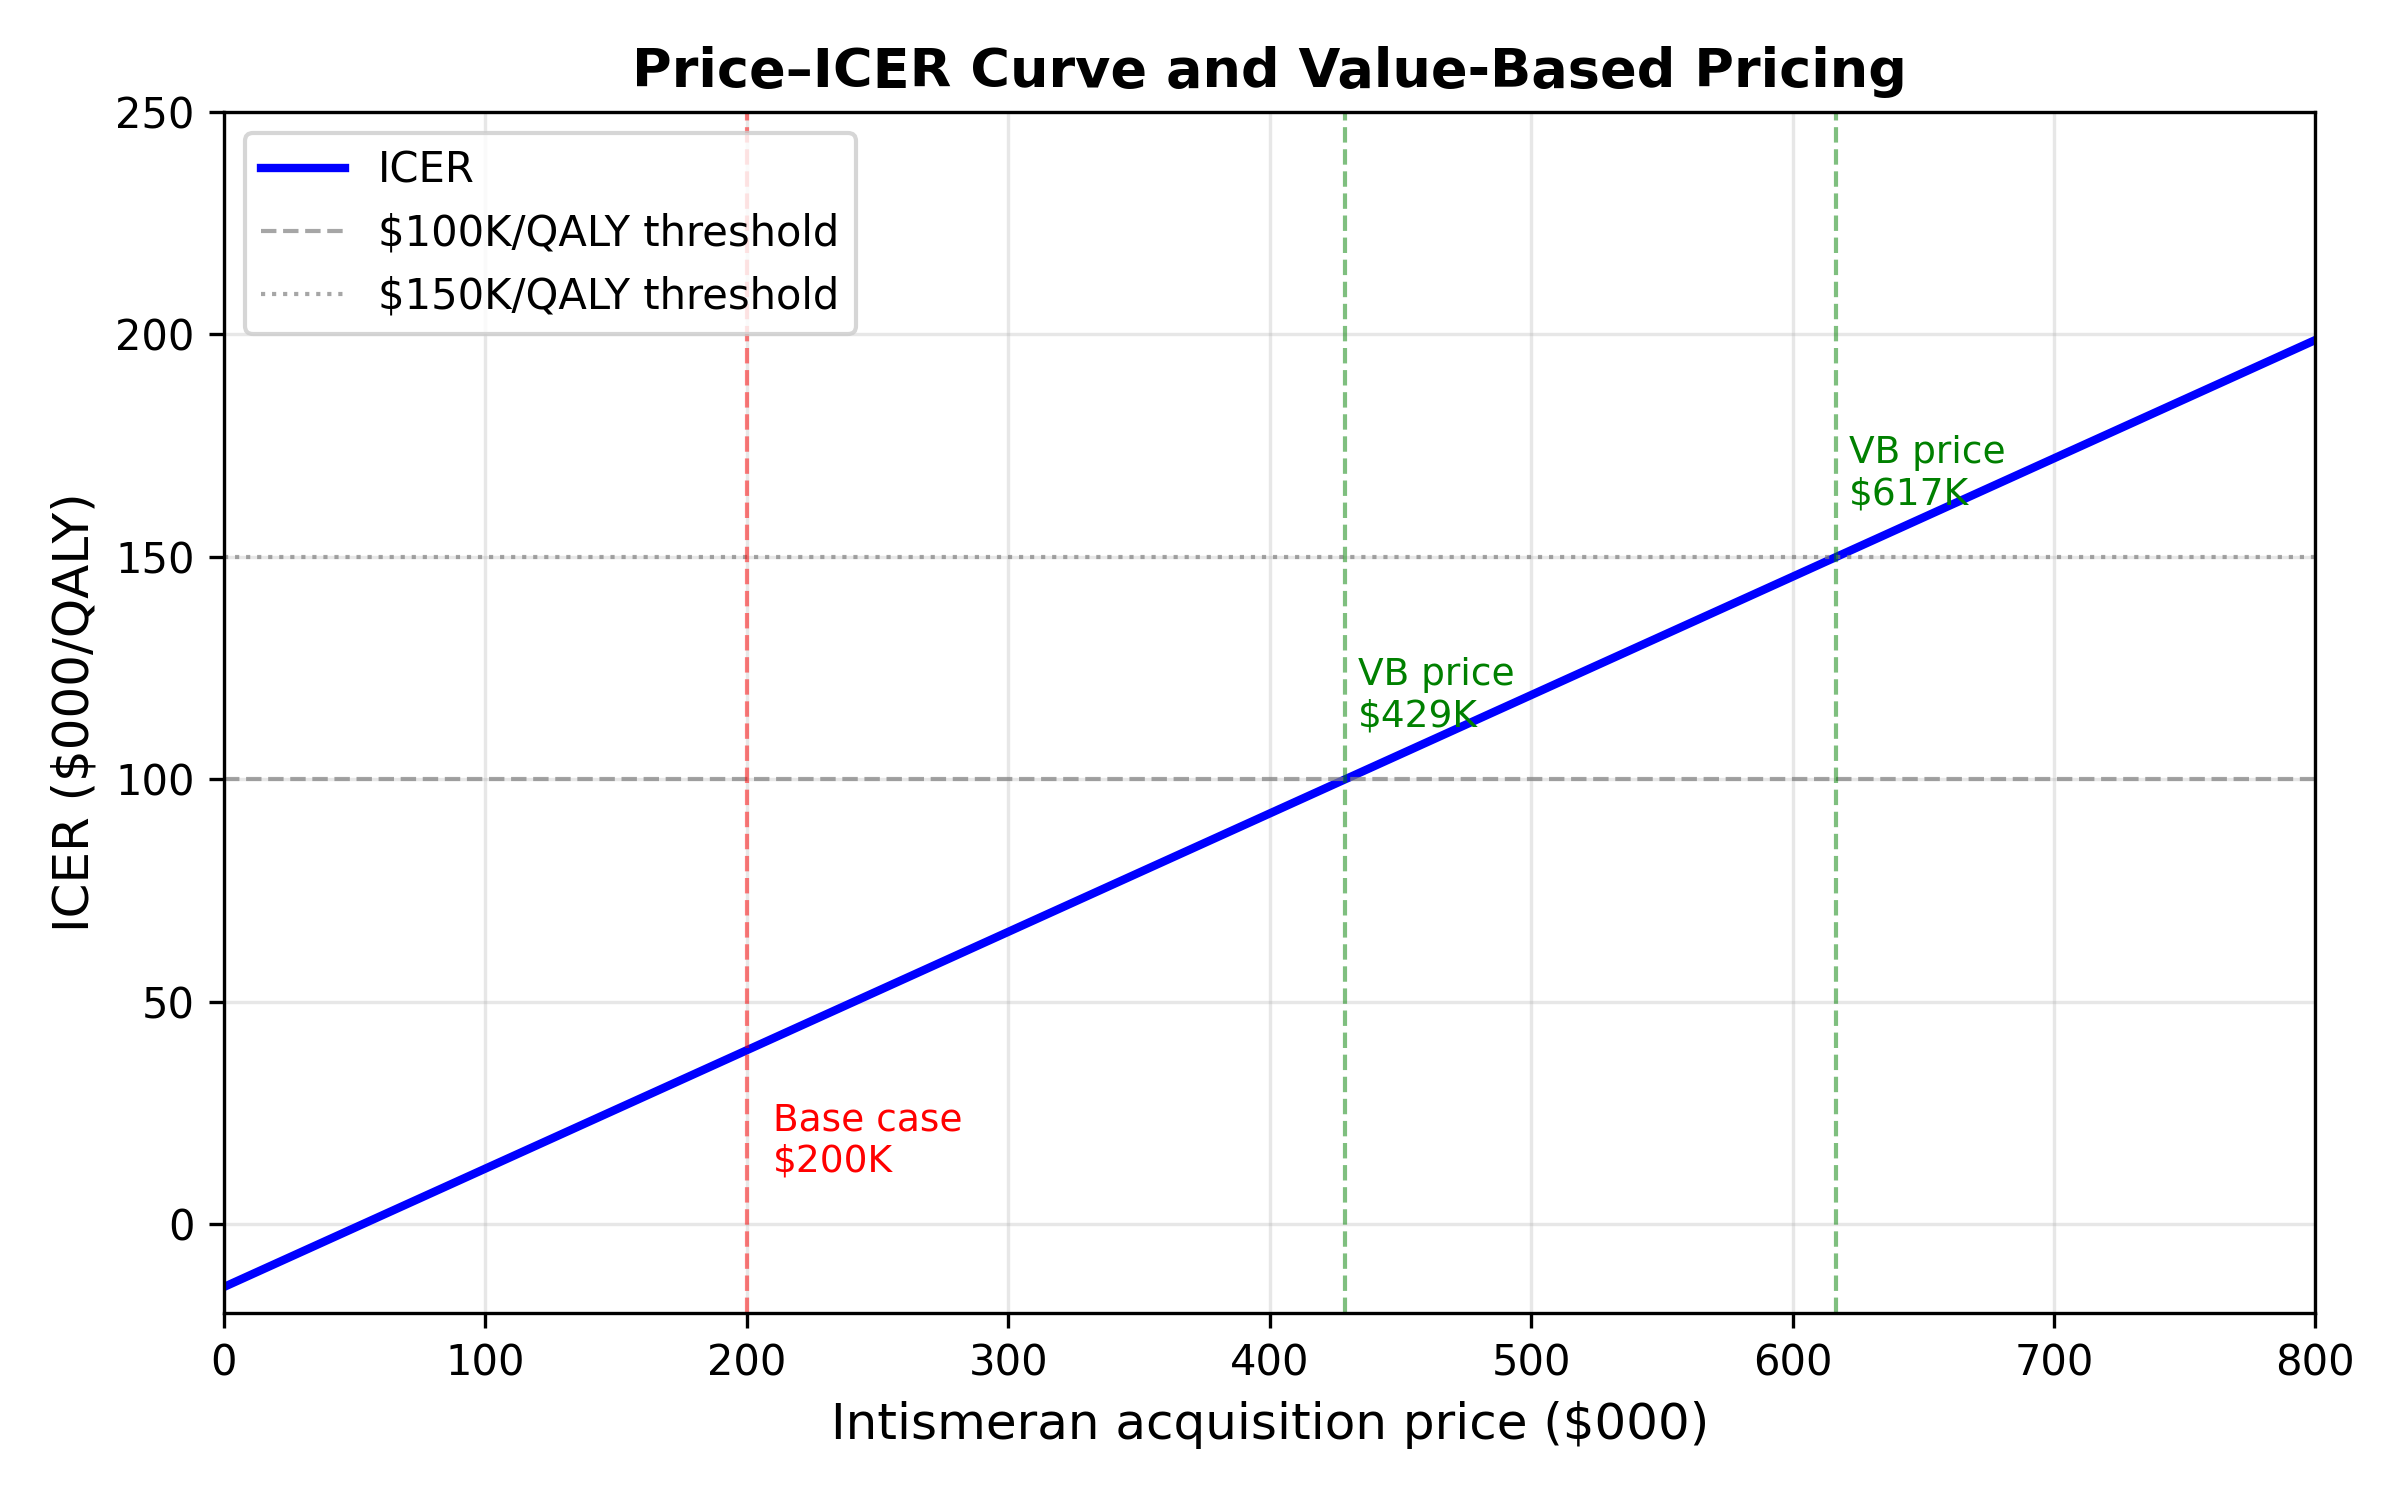
\includegraphics[width=\textwidth]{fig4_price_icer.png}
\caption{Price--ICER curve and value-based pricing. Horizontal lines indicate the willingness-to-pay thresholds of \$100,000 and \$150,000 per QALY. Vertical dashed lines show the base-case price (\$200,000), the deterministic threshold price at \$100,000/QALY (approximately \$429,000), and the deterministic threshold price at \$150,000/QALY (approximately \$616,000).}
\label{fig:price_icer}
\end{figure}

\subsection{Structural Scenario Analyses}

Scenario analysis results are summarized in Table~\ref{tab:scenarios}.

\begin{table}[H]
\centering
\caption{Scenario and Value-Based Price Thresholds}
\label{tab:scenarios}
\small
\setlength{\tabcolsep}{4pt}
\begin{tabularx}{\textwidth}{@{}>{\raggedright\arraybackslash}Xrrrr@{}}
\toprule
\textbf{Scenario} & \textbf{$\Delta$ Cost} & \textbf{$\Delta$ QALY} & \textbf{ICER} & \textbf{NMB @ \$150K} \\
\midrule
Base case (GP-constrained) & \$146,961 & 3.76 & \$39,105 & \$416,757 \\
\addlinespace
\multicolumn{5}{c}{\textit{Pricing}} \\
Price: \$100K/course & \$46,961 & 3.76 & \$12,496 & \$516,757 \\
Price: \$300K/course & \$246,961 & 3.76 & \$65,714 & \$316,757 \\
Price: \$500K/course & \$446,961 & 3.76 & \$118,932 & \$116,757 \\
\addlinespace
\multicolumn{5}{c}{\textit{Alternative assumptions}} \\
Weibull OS & \$293,679 & 5.35 & \$54,921 & \$508,411 \\
Discount rate: 0\% & \$183,728 & 5.91 & \$31,092 & \$702,636 \\
Discount rate: 5\% & \$136,896 & 2.86 & \$47,814 & \$292,571 \\
Time horizon: 10 years & \$95,573 & 1.28 & \$74,945 & \$95,714 \\
Time horizon: 20 years & \$115,739 & 2.91 & \$39,734 & \$321,191 \\
General population utilities & \$146,961 & 3.59 & \$40,970 & \$391,092 \\
\addlinespace
\multicolumn{5}{c}{\textit{Treatment-effect persistence}} \\
Treatment-effect waning (5\textendash10y hazard convergence) & \$224,317 & 2.13 & \$105,360 & \$95,042 \\
No direct OS benefit & \textendash\$14,562 & 0.50 & \textendash\$29,379 & \$88,915 \\
\bottomrule
\end{tabularx}
\end{table}

\subsection{Value-Based Price Thresholds}

The deterministic threshold price of intismeran was estimated by identifying the price at which the ICER reaches conventional willingness-to-pay thresholds (Table~\ref{tab:scenarios}). At the estimated acquisition cost of \$200,000 per course, the ICER was \$39,105/QALY. The deterministic threshold price at a \$100,000/QALY threshold was approximately \$429,000 per course, meaning the ICER remains below \$100,000/QALY even at more than twice the current estimated price. At a \$150,000/QALY threshold, the deterministic threshold price was approximately \$616,000 per course.



\section{Discussion}

\subsection{Principal Findings}

This early economic evaluation demonstrates that intismeran plus pembrolizumab is likely cost-effective for adjuvant treatment of resected stage IIIB--IV melanoma at conventional US willingness-to-pay thresholds. The base case ICER of \$39,105/QALY, the 3.76 QALY gain, and the 93.7\% probability of cost-effectiveness at \$100,000/QALY (98.2\% at \$150,000/QALY) all support this conclusion.

The economic value of the combination is generated through two complementary mechanisms described in detail below (Section~4.2): extended recurrence-free quality-adjusted survival and downstream cost offsets from avoided distant metastasis. The ICER is notably lower than the \$75,206 from the prior exploratory analysis \cite{mclean2024} (Section~4.5), reflecting the combined effect of mature clinical data and a structurally more conservative modelling framework.

\subsection{Economic Drivers and Cost Offsets}

The incremental \$146,961 lifetime cost of intismeran plus pembrolizumab is substantially lower than the \$200,000 acquisition cost of the intismeran course alone, because \$82,734 in downstream distant-metastasis management costs are avoided (combo \$342,542 vs pembro \$425,276). The QALY decomposition (Table~\ref{tab:base}) shows that the 3.76 incremental QALYs are driven almost entirely by additional time in the recurrence-free health state: the combination arm generates 3.83 more RF QALYs, partially offset by 0.32 fewer DM QALYs, with a small net gain of 0.24 LR QALYs. This asymmetry --- a large QALY gain concentrated in the least costly health state, paired with cost savings from the most costly state --- is the structural mechanism behind the favourable ICER.

The economic value is therefore not simply a matter of ``large QALY gain offsets upfront cost.'' The combination works through two pathways simultaneously: (i) it shifts patients from DM to RF, the highest-utility, lowest-cost state; and (ii) it compresses the time spent in DM, the highest-cost state, generating direct cost offsets. The ICER is low because the incremental expenditure is coupled to a large gain in recurrence-free quality-adjusted survival and to partial avoidance of the high cost of metastatic disease, not because the intervention is inexpensive.

\subsection{Pricing and Reimbursement Implications}

The base case assumes an intismeran acquisition price of \$200,000 per course, based on Jefferies analyst estimates. At this price, the ICER of \$39,105/QALY is well below conventional US thresholds. The value-based price analysis (Section~3.6) shows that the ICER remains below \$100,000/QALY at intismeran prices up to approximately \$429,000 per course and below \$150,000/QALY up to approximately \$616,000 per course, providing substantial headroom for price negotiations.

While individualized production requirements --- including tumor sequencing, mRNA synthesis, lipid nanoparticle formulation, and quality assurance for each batch --- may contribute to acquisition-price pressure, production cost and commercial price are distinct quantities. The \$200,000 estimate reflects the expected market price at launch, not the manufacturer's cost of goods sold. Several factors may reduce future production costs: sequencing costs continue to decline \cite{schwarze2020}, mRNA platform manufacturing is becoming increasingly standardized, and automation of the synthesis and formulation pipeline could reduce per-batch costs. However, whether these technical efficiencies will translate into lower acquisition prices for payers is uncertain, as pricing decisions are influenced by clinical value, competitive dynamics, and reimbursement negotiations, not solely by production economics.

Cost-effectiveness should not be conflated with affordability. The deterministic threshold price of approximately \$429,000 per course at \$100,000/QALY implies that the combination could be considered cost-effective at more than twice the current estimated price, but the incremental per-patient budget impact of adding \$200,000 in drug costs to an already expensive pembrolizumab regimen would be substantial in a population of eligible patients. Formal budget-impact analysis is needed alongside cost-effectiveness evidence for reimbursement decision-making.

\subsection{Long-Term Survival and Structural Uncertainty}

Long-term survival extrapolation is the dominant source of structural uncertainty in this analysis. The mature 5-year RFS and DMFS data from KEYNOTE-942 provide a robust foundation for the recurrence and metastasis components of the model, but OS remains exploratory (7 events per arm) and must be extrapolated to a lifetime horizon.

The necessity of the general population mortality constraint is best illustrated by comparing the constrained and unconstrained models. Without the GP mortality floor, the log-normal survival fit for the combination arm predicts a 30-year OS of 79.1\%, far exceeding the age- and sex-matched general population survival of 22.1\% at 30 years for the modeled cohort. This is implausible: a cohort of patients with resected stage IIIB--IV melanoma cannot have a lower mortality rate than the general population. Applying the GP mortality floor from 60 months onward --- a standard practice recommended by NICE DSU TSD 14 \cite{latimer2011} and used in published melanoma CEAs \cite{zhang2023} --- reduces the 30-year combination OS to 21.5\%, a clinically plausible trajectory. The constraint increases the ICER from \$51,753 (unconstrained) to \$39,105 (GP-constrained); the direction of this change is non-intuitive (the constraint reduces the ICER) because the unconstrained model predicts implausibly high survival for both arms, with a larger absolute gain for the combination arm.

The OS uncertainty is further underscored by the treatment-effect waning scenario. When the combination's recurrence-related hazard is allowed to converge to the pembrolizumab level between years 5 and 10, the ICER rises to \$105,360/QALY --- nearly three times the base case --- because the QALY gain is compressed from 3.76 to 2.13 while the incremental cost remains high. The range from \$39,105 to \$105,360 represents the plausible interval for the ICER under alternative persistence assumptions.

Finally, the choice of parametric distribution, while important, is secondary to the structural scenarios. The log-normal distribution was selected by AIC for the combination OS curve and was applied uniformly across all components for parsimony. However, AIC measures fit within the observed 5-year follow-up; it does not establish long-term clinical validity. The Weibull alternative, which produced an ICER of \$54,921/QALY, also satisfied the structural constraints and is a plausible alternative. The most informative bounds on the ICER come not from alternative parametric forms but from the treatment-effect waning and no-direct-OS-benefit scenarios, which directly address the question: what if the treatment effect does not persist? The best AIC-ranked mixed-family combination (OS: log-normal/Weibull, r$_{\text{DM}}$: log-normal/log-logistic, r$_{\text{LR}}$: log-logistic/Weibull) produced an ICER of \$56,460, consistent with the Weibull scenario and within the range of structural uncertainty, further supporting the robustness of the base-case conclusion.

\subsection{Comparison with Previous Economic Evaluations}

Direct comparison of ICERs across adjuvant melanoma cost-effectiveness studies is not straightforward, because the incremental decision differs. Bensimon et al.\ \cite{bensimon2019} and Zhang et al.\ \cite{zhang2023} evaluated pembrolizumab versus observation, estimating the value of adding immunotherapy to surveillance. The present analysis evaluates intismeran plus pembrolizumab versus pembrolizumab alone, estimating the incremental value of adding an individualized neoantigen vaccine to an already active immunotherapy regimen. The relevant policy question is therefore not whether the combination is cost-effective in absolute terms, but whether the combination of two active agents can provide sufficient additional value --- through both clinical benefit and downstream cost offsets --- to justify the cost of the second agent.

The ICER of \$39,105/QALY is within the range of published estimates for the initial pembrolizumab decision (\$38,050--\$78,400/QALY), but this comparability is coincidental rather than meaningful. The absolute QALY gain from adding intismeran to pembrolizumab (3.76 QALYs) is larger than the gain from adding pembrolizumab to observation (1.2--2.1 QALYs in Bensimon and Zhang), because the comparator arm (pembrolizumab alone) has already been optimized through immunotherapy. The incremental cost is also larger (\$146,961 vs approximately \$100,000--\$150,000). The ratio happens to fall within a similar range because both numerator and denominator increase proportionally, not because the value proposition is comparable.

The comparison with the 2024 exploratory analysis \cite{mclean2024} is more informative but requires careful interpretation. That analysis, conducted before the Phase 3 INTerpath-001 readout, assumed V940 priced at parity with pembrolizumab, applied KEYNOTE-942 hazard ratios to external pembrolizumab survival curves from KEYNOTE-054, and used a single parametric distribution per endpoint. The present analysis differs on all four dimensions: post-Phase III evidence context, direct fitting to KEYNOTE-942 5-year data, a \$200,000 price assumption, and a ratio-constrained structural framework with a general population mortality floor. The lower ICER (\$39,105 vs \$75,206) is the net result of these four differences, not a univariate effect of any single factor, and should not be interpreted as evidence that intismeran is simply more effective than previously estimated.

\subsection{Clinical and External Validity}

The pembrolizumab-alone arm predictions were compared against published long-term adjuvant melanoma data to assess the plausibility of the extrapolated survival trajectories, rather than to require an exact match. The KEYNOTE-942 trial enrolled a higher-risk population (stage IIIB--IV, including resected stage IV) than KEYNOTE-054 (stage IIIA--C) and CheckMate 238 (stage IIIB--IV, but with different entry criteria). The model's lower 7-year RFS for the pembrolizumab arm (31.7\% vs 50\% in KEYNOTE-054) is therefore expected and reflects the underlying risk differences rather than a failure of calibration. The model correctly reproduces the 5-year OS and DMFS of the pembrolizumab arm, supporting the structural validity of the PSM framework.

No external long-term data exist for the combination arm (first-in-class therapy). The positive Phase 3 INTerpath-001 readout provides directional confirmation of the clinical benefit of intismeran plus pembrolizumab, but the numerical hazard ratios have not yet been disclosed, and the extent to which Phase 3 results will align with the Phase 2b KEYNOTE-942 estimates used in this model remains to be determined. Two structural scenarios address the uncertainty in the combination arm: (i) the treatment-effect waning scenario (ICER \$105,360/QALY); and (ii) the no-direct-OS-benefit scenario, an OS-neutral structural scenario in which intismeran plus pembrolizumab remained dominant (lower cost and higher QALY) compared with pembrolizumab alone, indicating that the base-case conclusion does not rely on a direct OS benefit but can be supported by recurrence prevention alone.

\subsection{Limitations}

This analysis has several limitations that should be considered when interpreting the results. First, the Phase 3 INTerpath-001 trial has reported only topline results; numerical hazard ratios and subgroup data have not yet been disclosed, and all quantitative efficacy inputs are derived from the Phase 2b KEYNOTE-942 trial. Second, overall survival data from KEYNOTE-942 remain exploratory, with only 7 events per arm at the 5-year analysis, and the 5-year OS estimate of 92.2\% versus 71.3\% should be interpreted with caution. Third, survival curves were reconstructed from published Kaplan--Meier figures using digitized coordinates rather than being estimated from individual patient-level data, which introduces measurement error in the parametric fits. Fourth, survival extrapolation beyond the observed 5-year follow-up, while structurally constrained and anchored to a general population mortality floor, remains sensitive to the choice of parametric distribution and the assumption that the treatment effect persists indefinitely. Fifth, the intismeran acquisition price of \$200,000 per course is based on analyst estimates, and the actual market price may differ. Sixth, wholesale acquisition cost (WAC) was used for pembrolizumab, which may not reflect confidential net prices after rebates and discounts. Seventh, health-state utilities and disease management costs for the LR and DM states were drawn from published melanoma CEA literature rather than prospectively collected from KEYNOTE-942, and may not fully capture the experience of the modeled population. Eighth, indirect costs, productivity losses, and informal caregiver burden were not included, which may underestimate the societal value of preventing recurrence and distant metastasis in a working-age population. Ninth, no formal budget-impact analysis was conducted; the cost-effectiveness findings should be complemented by an affordability assessment when pricing and population-level data become available. Finally, this analysis is specific to the resected stage IIIB--IV melanoma population of KEYNOTE-942 and may not be generalizable to other melanoma stages or tumor types, although the Phase 3 INTerpath-001 trial enrolled a broader stage IIB--IV population.

\subsection{Conclusion}

Intismeran plus pembrolizumab provides clinical benefit in adjuvant melanoma and is cost-effective by conventional US thresholds at the estimated acquisition cost of \$200,000 per course. The deterministic threshold price analysis shows that the ICER remains below \$100,000/QALY at intismeran prices up to approximately \$429,000 per course, providing substantial headroom for price negotiations. The QALY gain from the combination, driven by improved recurrence-free survival and reduced distant metastases, partially offsets the upfront cost of individualized therapy. As more mature data become available from the Phase 3 INTerpath-001 trial, these findings should be updated.\section*{Declarations}

\textbf{Conflict of interest:} The author declares no competing interests relevant to this study.

\textbf{Reporting:} This study adheres to the Consolidated Health Economic Evaluation Reporting Standards 2022 (CHEERS 2022) \cite{husereau2022} (Supplementary Checklist).

\textbf{Data availability:} All data used in this analysis are derived from published sources cited in the references. The model code is available at \url{https://github.com/yichao2022/cea-intismeran}.

\textbf{Code availability:} The partitioned survival model was implemented in Python and is available at \url{https://github.com/yichao2022/cea-intismeran}.

\textbf{Author contributions:} Yichao Jin conceived and designed the study, developed the model, conducted the analysis, and wrote the manuscript.

% --- References ---
\newpage
\bibliography{refs}

\end{document}